\section{Auswertung}
\label{sec:Auswertung}
Die Werte der Bauteile in der untersuchten Schaltung betragen
\begin{align*}
  L &= \SI{10,11(003)}{\milli\henry}\,, \\
  C &= \SI{2,098(0006)}{\nano\farad}\,, \\
  R_1 &= \SI{48,1(01)}{\ohm}\,, \\
  R_2 &= \SI{509,5(05)}{\ohm}\,. \\
\end{align*}
\subsection{Ermittlung der Widerstände $R_\text{eff}$ des Schwingfalls und $R_\text{ap}$ des aperiodischen Grenzfalls}
Für jegliche Messungen und Berechnungen wird ab hier der Widerstand $R_1$ verwendet.
Die mit dem Oszilloskop aufgenommene Spannung am Kondensator bei der gedämpften
Schwingung ist in Abbildung \ref{fig:einhuellende} zu sehen. Dort ist auch
bereits die Einhüllende eingezeichnet.

\begin{figure}
  \centering
  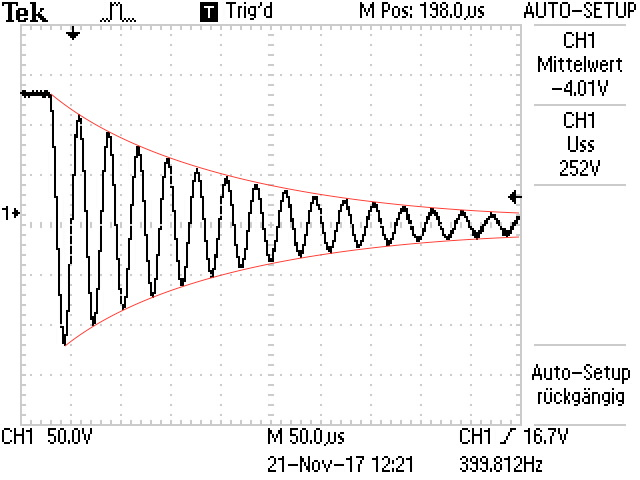
\includegraphics[width=300pt]{data/gedaempfte_schwingung2.JPG}
  \caption{Aufnahme des Spannungsverlaufs am Kondensator und Einhüllende bei der
  gedämpften Schwingung}
  \label{fig:einhuellende}
\end{figure}

Alle Spannungen am Oszilloskop wurden mit zehn multipliziert dargestellt. Die
aus der Kurve entnommenen Messwerte sind in Tabelle \ref{tab:einhuellende} eingetragen.

\begin{table}
\centering
\caption{Messdaten zur gedämpften Schwingung des Schwingkreises}
\label{tab:einhuellende}
\begin{tabular}{c c c}
\toprule
$t/$µs & $10U_\mathrm{C}/$V & $U_\mathrm{C}/$V \\
\midrule
  1 & 132 & 13,2 \\
 29 & 112 & 11,2 \\
 58 &  94 &  9,4 \\
 88 &  80 &  8,0 \\
118 &  66 &  6,6 \\
147 &  58 &  5,8 \\
177 &  50 &  5,0 \\
206 &  42 &  4,2 \\
236 &  36 &  3,6 \\
265 &  30 &  3,0 \\
297 &  28 &  2,8 \\
324 &  24 &  2,4 \\
354 &  20 &  2,0 \\
382 &  18 &  1,8 \\
412 &  16 &  1,6 \\
441 &  14 &  1,4 \\
\bottomrule
\end{tabular}
\end{table}

Es wird eine nichtlineare Ausgleichsrechnung mit diesen Messwerten durchgeführt.
In diesem Fall gilt $U(t) \propto I(t)$ gemäß \eqref{eqn:ifunktion}, sodass die
Ausgleichsfunktion der Zuordnung
\begin{equation}
  U_\text{C}(t) = U_0 \exp(-2 \pi \mu t)
\end{equation}
folgt. Dabei gilt für µ der Zusammenhang
\begin{equation}
  \mu = \frac{R}{4 \pi L}\,.
  \label{eqn:mu}
\end{equation}
Der Widerstand R wird hier mit dem effektiven Dämpfungswiderstand $R_\text{eff}$ assoziiert, der
durch die Ausgleichsrechnung aus $\mu$ bestimmt werden kann.
In Abbildung \ref{fig:einhuellendefit} sind die abgelesenen Messwerte und der Graph
der konkreten Ausgleichsfunktion zu sehen.

\begin{figure}
  \centering
  \includegraphics{build/einhuellende.pdf}
  \caption{Auftragung der Kondensatorspannung gegen die Zeit und Graph der Ausgleichsfunktion}
  \label{fig:einhuellendefit}
\end{figure}

Die Parameter ergeben sich hier zu
\begin{align*}
  U_0 &= \SI{13,04(011)}{\volt}\,, \\
  \mu &= \SI{861(12)}{\micro\second}\,,
\end{align*}
sodass für den effektiven Dämpfungswiderstand $R_\text{eff}$ nach \eqref{eqn:mu}
\begin{equation*}
  R_\text{eff} = \SI{109,4(16)}{\ohm}
\end{equation*}
folgt. Die relative Unsicherheit beträgt 1,46\%. Die charakteristische
Abklingdauer $T_\text{ex}$ ist mit \eqref{eqn:abklingdauer} und \eqref{eqn:mu} dann
\begin{equation*}
  T_\text{ex} = \frac{2L}{R} = \frac{1}{2\pi \mu} = \SI{184,8(26)}{\micro\second}
\end{equation*}
mit einer relativen Unsicherheit von 1,41\%.

Es ist auffällig, dass der experimentell bestimmte Wert $R_\text{eff}$ vom Wert $R_1$ des verwendeten
Widerstands um ungefähr $\SI{50}{\ohm}$ abweicht. Dies ist jedoch genau der Innenwiderstand
des verwendeten Generators. Deswegen wird dieser ab sofort bei allen Berechnungen zu dem
gegebenen Widerstand addiert.

Für den aperiodischen Grenzfall muss ein Widerstand $R_\text{ap}$ eingestellt werden.
Dieser wurde zu $\SI{3,550}{\kilo\ohm}$ bestimmt. Wird dieser Widerstand nach
\eqref{eqn:rap} bestimmt, so ergibt sich für ihn $\SI{4,390(0009)}{\kilo\ohm}$.
Dabei beträgt die absolute Unsicherheit $\SI{-840(9)}{\kilo\ohm}$.

\subsection{Bestimmung der Güte und der Breite der Resonanzkurve für erzwungene Schwingungen}
Bei allen Messungen und Berechnungen wird ab hier der Widerstand $R_2$ verwendet,
auf diesen wird der Generatorinnenwiderstand von $\SI{50}{\ohm}$ addiert.

Wie an \eqref{eqn:Ucfrequenz} ersichtlich ist, hängt die Kondensatorspannung von
der Frequenz ab. In den Tabellen \ref{tab:amplitude1} und \ref{tab:amplitude2} sind die aufgenommenen Messwerte
angegeben, die untersucht werden sollen. Dabei ist $U_\text{C}$ die Kondensatorspannung,
$U$ ist die durch den frequenzgängigen Tastkopf gemessene Generatorspannung.
Es sei darauf hingewiesen, dass ursprünglich Messwerte bereits ab einer
Frequenz von $\SI{10}{\hertz}$ genommen wurden. Diese tragen jedoch keine
signifikante Information, da für sie durchgängig $U_\text{C}/U \approx 1$ gilt.
Daher werden sie nicht weiter betrachtet. Die nicht verwendeten Messwerte können
bei Bedarf im Anhang eingesehen werden.

\begin{table}
\centering
\caption{Messdaten zur Frequenzabhängigkeit der Kondensatorspannung}
\label{tab:amplitude1}
\begin{tabular}{c c c c c c}
\toprule
$f/$kHz & $10U_\mathrm{C}/$V & $U_\mathrm{C}/$V & $10U$/V & $U$/V & $U_\mathrm{C}/U$ \\
\midrule
  0,5	&  64,8  &  6,48 & 65   & 6,5 & 0,997 \\
  0,6	&  64,8  &  6,48 & 64   & 6,4 & 1,012 \\
  0,7	&  64,8  &  6,48 & 64   & 6,4 & 1,012 \\
  0,8	&  64,8  &  6,48 & 64   & 6,4 & 1,012 \\
  0,9	&  64,8  &  6,48 & 64   & 6,4 & 1,012 \\
  1	  &  66	   &  6,6  & 63,5 & 6,35& 1,039 \\
  1,5	&  66	   &  6,6  & 64,5 & 6,45& 1,023 \\
  2	  &  66	   &  6,6  & 64,5 & 6,45& 1,023 \\
  3	  &  66,8	 &  6,68 & 66   & 6,6 & 1,012 \\
  4	  &  66,8	 &  6,68 & 64   & 6,4 & 1,044 \\
  5	  &  67,6	 &  6,76 & 64   & 6,4 & 1,056 \\
  6	  &  67,6	 &  6,76 & 64,5 & 6,45& 1,048 \\
  7	  &  68,4	 &  6,84 & 65   & 6,5 & 1,056 \\
  8	  &  69,2	 &  6,92 & 65   & 6,5 & 1,065 \\
  9	  &  70,8	 &  7,08 & 65   & 6,5 & 1,089 \\
 10	  &  72	   &  7,20 & 63,5 & 6,35& 1,133 \\
 15	  &  81	   &  8,1  & 64,5 & 6,45& 1,256 \\
 20	  &  98	   &  9,8  & 64,5 & 6,45& 1,519 \\
 21	  & 103	   & 10,3  & 64,5 & 6,45& 1,597 \\
 22	  & 108	   & 10,8  & 64,5 & 6,45& 1,674 \\
 23	  & 115	   & 11,5  & 64,5 & 6,45& 1,783 \\
 24	  & 121	   & 12,1  & 64,5 & 6,45& 1,876 \\
 25	  & 131	   & 13,1  & 63,5 & 6,35& 2,063 \\
 26	  & 140	   & 14,0  & 63,5 & 6,35& 2,205 \\
 27	  & 151	   & 15,1  & 63,5 & 6,35& 2,378 \\
 28	  & 165	   & 16,5  & 63,5 & 6,35& 2,598 \\
 29	  & 181	   & 18,1  & 63,5 & 6,35& 2,850 \\
 30	  & 197	   & 19,7  & 63,5 & 6,35& 3,102 \\
 31	  & 212	   & 21,2  & 63,5 & 6,35& 3,339 \\
 32	  & 230	   & 23    & 63,5 & 6,35& 3,622 \\
 33	  & 238	   & 23,8  & 63,5 & 6,35& 3,748 \\
 34	  & 234	   & 23,4  & 63,5 & 6,35& 3,685 \\
 35	  & 222	   & 22,2  & 64   & 6,4 & 3,469 \\
 36	  & 202	   & 20,2  & 64   & 6,4 & 3,156 \\
 37	  & 180	   & 18    & 64   & 6,4 & 2,813 \\
 38	  & 160	   & 16    & 64   & 6,4 & 2,500 \\
 39	  & 140	   & 14    & 64   & 6,4 & 2,188 \\
 40	  & 128	   & 12,8  & 64   & 6,4 & 2,000 \\
\bottomrule
\end{tabular}
\end{table}

\begin{table}
\centering
\caption{Messdaten zur Frequenzabhängigkeit der Kondensatorspannung (Fortsetzung)}
\label{tab:amplitude2}
\begin{tabular}{c c c c c c}
\toprule
$f/$kHz & $10U_\mathrm{C}/$V & $U_\mathrm{C}/$V & $10U$/V & $U$/V & $U_\mathrm{C}/U$ \\
\midrule
 41	  & 115	   & 11    & 64   & 6,4 & 1,797 \\
 42	  & 103	   & 10,3  & 64   & 6,4 & 1,609 \\
 43	  &  93	   &  9,3  & 64   & 6,4 & 1,453 \\
 44	  &  85	   &  8,5  & 64   & 6,4 & 1,328 \\
 45	  &  77	   &  7,7  & 64   & 6,4 & 1,203 \\
 46	  &  72	   &  7,2  & 64   & 6,4 & 1,125 \\
 47	  &  63,6  &  6,36 & 64   & 6,4 & 0,938 \\
 48	  &  59,2  &  5,92 & 64   & 6,4 & 0,925 \\
 49	  &  54,8	 &  5,48 & 64   & 6,4 & 0,856 \\
 50	  &  51,6	 &  5,16 & 64   & 6,4 & 0,806 \\
 60	  &  30	   &  3    & 64   & 6,4 & 0,469 \\
 70	  &  19,4	 &  1,94 & 64   & 6,4 & 0,303 \\
 80	  &  13,7	 &  1,37 & 64   & 6,4 & 0,214 \\
 90	  &  10,4	 &  1,04 & 64   & 6,4 & 0,163 \\
100 	&   8,1	 &  0,81 & 64   & 6,4 & 0,127 \\
150	  &   2,91 &	0,29 & 64   & 6,4 & 0,045 \\
200	  &   1,4	 &  0,14 & 64   & 6,4 & 0,022 \\
300	  &   0,29 &	0,03 & 64   & 6,4 & 0,005 \\
\bottomrule
\end{tabular}
\end{table}

In Abbildung \ref{fig:amplitudelog} ist die Kondensatorspannung relativ
zur Generatorspannung in Abhängigkeit der Frequenz dargestellt. Die Achse, auf der
die Frequenz aufgetragen ist, ist logarithmisch skaliert.

\begin{figure}
  \centering
  \includegraphics{build/amplitudelog.pdf}
  \caption{Halblogarithmische Auftragung der normierten Kondensatorspannung gegen die Frequenz}
  \label{fig:amplitudelog}
\end{figure}

Aus dem Diagramm und den Messwerten lässt sich die Güte, die die maximale
Überhöhung der Amplitude angibt, zu ungefähr
\begin{equation*}
  q_\text{exp} = 3,748
\end{equation*}
bestimmen. Der theoretische Wert ergibt sich durch Berechnung mit \eqref{eqn:guete}
zu
\begin{equation*}
  q_\text{theo} = \SI{3,923(0009)}\,,
\end{equation*}
wobei für $R$ der Wert $R_2+\SI{50}{\ohm}$ eingesetzt wird.
Die relative Messabweichung beträgt dann 4,46\%.
Der Bereich, in dem die Resonanz auftritt, wird in Abbildung \ref{fig:amplitudelin}
linear dargestellt, um den Bereich der Resonanz besser zu veranschaulichen.

\begin{figure}
  \centering
  \includegraphics{build/amplitudelin.pdf}
  \caption{Lineare Auftragung der normierten Kondensatorspannung gegen die Frequenz um den Resonanzbereich}
  \label{fig:amplitudelin}
\end{figure}

Die Breite der Resonanzkurve $f_{+} - f_{-}$\footnote{Hier wird die Breite in der
Frequenz betrachtet statt in der Kreisfrequenz. Dies erscheint sinnvoll, da am
Generator stets eine Frequenz und nicht die Kreisfrequenz eingestellt wurde.},
definiert analog zu den Erklärungen zu \eqref{eqn:breite}, ergibt sich experimentell zu
\begin{equation*}
  (f_{+} - f_{-})_\text{exp} = (37,5-28,25)\,\text{Hz} = \SI{9,25}{\kilo\hertz}\,.
\end{equation*}
Der nach der Theorie zu erwartende Wert beträgt nach der zuvor angegebenen Gleichung
\begin{equation*}
  (f_{+} - f_{-})_\text{theo} = \frac{R_2+\SI{50}{\ohm}}{2\pi L} = \SI{8,808(27)}{\kilo\hertz}\,.
\end{equation*}
Die relative Abweichung zu diesem Wert ist 4,77\%.

\subsection{Untersuchung der Frequenzabhängigkeit der Phasenverschiebung im angeregten Schwingkreis}

Der gemessene Abstand $a$ zwischen den Nulldurchgängen der Kondensator- und Generatorspannung
sowie die daraus nach \eqref{eqn:ab2phi} ermittelte Phasenverschiebung bei eingestellter Frequenz zwischen ihnen sind
in den Tabellen \ref{tab:phase1} und \ref{tab:phase2} zu sehen.

\begin{table}
\centering
\caption{Messdaten zur Phasenverschiebung zwischen Kondensator- und Generatorspannung}
\label{tab:phase1}
\begin{tabular}{c c c}
\toprule
$f/$kHz & $a/$µs & $\phi/$rad \\
\midrule
 0,01	 & 9200    & 0,58 \\
 0,02	 & 2400    & 0,30 \\
 0,03	 & 1080    & 0,20 \\
 0,04	 &  540    & 0,14 \\
 0,05	 &  500    & 0,16 \\
 0,06	 &  360    & 0,14 \\
 0,07	 &  260    & 0,11 \\
 0,08	 &  208    & 0,10 \\
 0,09	 &  160    & 0,09 \\
 0,1	 &  148    & 0,09 \\
 0,125 &  127    & 0,10 \\
 0,15	 &   97    & 0,09 \\
 0,175 &   80    & 0,09 \\
 0,2	 &   68    & 0,09 \\
 0,225 &   57    & 0,08 \\
 0,25	 &   48    & 0,08 \\
 0,275 &   43    & 0,07 \\
 0,3	 &   39    & 0,07 \\
 0,4	 &   27    & 0,07 \\
 0,5	 &   21,2  & 0,07 \\
 0,6	 &   17,6  & 0,07 \\
 0,7	 &   15,2  & 0,07 \\
 0,8	 &   13,2  & 0,07 \\
 0,9	 &   11,2  & 0,06 \\
 1	   &   10,8  & 0,07 \\
 1	   &    7,2  & 0,07 \\
 2	   &    5,5  & 0,07 \\
 3	   &    4,1  & 0,08 \\
 4	   &    3,4  & 0,09 \\
 5	   &    2,8  & 0,09 \\
 6	   &    2,64 & 0,10 \\
 7	   &    2,44 & 0,11 \\
 8	   &    2,24 & 0,11 \\
 9	   &    2,16 & 0,12 \\
10	   &    2,0  & 0,13 \\
15	   &    1,52 & 0,14 \\
20	   &    1,84 & 0,23 \\
25	   &    2,48 & 0,39 \\
27	   &    3,08 & 0,53 \\
30	   &    4,16 & 0,78 \\
\bottomrule
\end{tabular}
\end{table}

\begin{table}
\centering
\caption{Messdaten zur Phasenverschiebung zwischen Kondensator- und Generatorspannung (Fortsetzung)}
\label{tab:phase2}
\begin{tabular}{c c c}
\toprule
$f/$kHz & $a/$µs & $\phi/$rad \\
\midrule
32	& 5,72 & 1,15 \\
34	& 7,5  & 1,60 \\
36	& 9,1  & 2,06 \\
38	& 9,8  & 2,34 \\
40	& 10   & 2,51 \\
45	& 9,6  & 2,71 \\
50	& 8,9  & 2,80 \\
60	& 7,9  & 2,98 \\
70	& 6,9  & 3,03 \\
80	& 6,1  & 3,07 \\
90	& 5,6  & 3,17 \\
100 & 5,12 & 3,22 \\
150 & 3,76 & 3,54 \\
\bottomrule
\end{tabular}
\end{table}

Die Phasenverschiebung $\phi$ wird in Abbildung \ref{fig:philog} gegen die Frequenz
$f$ aufgetragen. Die Frequenzachse wird erneut logarithmisch skaliert. Blau markierte
Punkte sind auf Messfehler zurückzuführende Ausreißer. Die Phasenverschiebung kann
nicht mehr als $\pi$ betragen.

\begin{figure}
  \centering
  \includegraphics{build/philog.pdf}
  \caption{Halblogarithmische Auftragung der Phasenverschiebung gegen die Frequenz}
  \label{fig:philog}
\end{figure}

Wie zuvor wird der relevante Bereich erneut in einem linear skalierten Diagramm
dargestellt. Aus Abbildung \ref{fig:philin} lassen sich dann zuverlässiger die Größen
$f_1$, $f_\text{res}$ und $f_2$, bei denen die Phasenverschiebung jeweils $\frac{\pi}{4}$,
$\frac{\pi}{2}$ und $\frac{3\pi}{4}$ beträgt, ablesen.

\begin{figure}
  \centering
  \includegraphics{build/philin.pdf}
  \caption{Lineare Auftragung der Phasenverschiebung gegen die Frequenz}
  \label{fig:philin}
\end{figure}

Die theoretischen Werte für die charakteristischen Frequenzen lassen sich durch
\eqref{eqn:omega12}, die Resonanzfrequenz durch \eqref{eqn:resonanzfrequenz} berechnen. In Tabelle \ref{tab:frequenzvergleich} werden experimentelle und theoretische
Werte aufgelistet und verglichen.
\begin{table}
\centering
\begin{tabular}{cccc}
\toprule
& $f_\mathrm{res}/$kHz & $f_1/$kHz & $f_2/$kHz \\
\midrule
Experiment & $33,8$ & $38,15$ & $30$\\
Theorie & $33,99 \pm 0,07 $ & $ 39,24 \pm 0,08$ & $30,43 \pm 0,06$ \\
\hline
relative Abweichung & 0,56\% & 2,78\% & 1,41\%\\
\bottomrule
\end{tabular}
\caption{Vergleich der experimentell ermittelten und theoretisch berechneten Werte für die Frequenzen $f_\mathrm{res}$ und $f_{1,2}$}
\label{tab:frequenzvergleich}
\end{table}
